\setAuthor{}
\setRound{piirkonnavoor}
\setYear{2019}
\setNumber{G 9}
\setDifficulty{9}
\setTopic{TODO}

\prob{Kiik}
Juku kiigub  nii suure hooga, et kiik jõuab haripunktis kiigepostide (kiige pöörlemistelje) kõrguseni. Suure hoo tõttu hakkab Juku muretsema, kas kiige postid ikka vastu peavad.\\
\osa Leida minimaalne ja maksimaalne jõud, mida Juku kiikumisel postidele avaldab.\\
\osa Leida minimaalne ja maksimaalne jõumoment, mida Juku kiikumisel postidele avaldab. Jõumoment arvutada kiigeposti alumise otsa ehk maasse kinnitamise punkti suhtes.
Kiige võll (pöörlemistelg) on kinnitatud kahe horisontaalse posti otsa kõrgusel $H$ maapinnast. Tasakaaluasendis on Juku masskeskme kõrgus maapinnast h. Juku mass on $m$, raskuskiirendus g. Kiige istme mass lugeda tühiseks. Lihtsustatult võib Jukut vaadelda punktmassina, mille kaugus kiige võllist ei muutu. 



\hint

\solu
\osa Minimaalne jõud: Haripunktis on Juku hetkeliselt vabalangemises ning mingit jõudu ei avalda. Seega on minimaalne jõud: 
$$F_{min} = 0 \quad\pp{1.5}$$ 
Maksimaalne jõud: Kiikumise ajal rakenduvad postidele 2 jõudu: Juku raskusjõud ning pöörlemisest tulev tsentrifugaaljõud. Mõlemad on maksimaalsed ning samasuunalised, kui kiik on vertikaalasendis \pp{0.5}. Olgu kiige pöörlemisraadius Juku masskeskme suhtes $R = H-h$. Kasutades energia jäävust kiige vertikaal- ja horisontaalasendi jaoks saame: 
$$mgR = \frac{mv^2}{2} \Rightarrow v^2 = 2gR \quad\pp{1}$$ 
Tsentrifugaaljõu valemist saame:
$$F_C = m\frac{v^2}{R} = m\frac{2gR}{R} = 2mg \quad\pp{1}$$ 
Summarne jõud:
$$F_{max} = F_C + F_R = 2mg + mg = 3mg \quad\pp{0.5}$$ 
\osa Minimaalne jõumoment: Kiige vertikaalasendis on jõuõlg kiigeposti alumise punkti suhtes $0$, seega minimaalne jõumoment:
$$\tau_{min} = 0\quad\pp{1}$$ 
Maksimaalne jõumoment: Kuna võll kõrgusel $H$ on ainuke kiige kinnituspunkt, rakendub kogu Juku poolt rakendatav jõud sellesse punkti \pp{0.5}. Jõumoment on maksimaalne, kui jõuõlg $H$ ning sellesse punkti rakenduv jõud on risti. Seega piisab maksimaalse horisontaalse jõu leidmisest. Tähistame kiige hetkeasukoha ja haripunkti tasandi vahelise kauguse $s$ ning nende vahelise nurga $\varphi$ (vt. joonis). Tsentrifugaaljõud on alati suunatud piki raadiust ning analoogselt maksimaalse jõu arvutusele saame energia jäävusest:
$$F_C = m\frac{2gs}{R} = 2mg\sin{\varphi}\quad\pp{1}$$ 
Lisaks tuleb arvestada raskusjõu raadiusesihilist komponenti $F_{R||} = F_R\sin{\varphi} = mg\sin{\varphi}\pp{1.5}*$.
Seega rakendub piki raadiust võllile jõud:
$$F_{||} = F_C + F_{R||} = 3mg\sin{\varphi}\quad\pp{0.5}*$$ 
Meid huvitab selle jõu horisontaalkomponent:
$$F_H = F_{||}\cos{\varphi} = 3mg\sin{\varphi}\cos{\varphi}\quad\pp{0.5}$$ 
Teades, et $\sin{2\varphi}=2\sin{\varphi}\cos{\varphi}$ saame:
$$F_H = \frac{3}{2}mg\sin{2\varphi}\quad\pp{1}$$ 
Siinuse maksimaalne väärtus on $1$, mille saame $\varphi = \ang{45}$ korral, mis on antud ülesande jaoks reaalne väärtus. Seega saame maksimaalseks horisontaalseks jõuks:
$$F_H = \frac{3}{2}mg\quad\pp{1}$$ 
Millele vastab maksimaalne jõumoment:
$$\tau_{max} = F_HH = \frac{3}{2}mgH\quad\pp{0.5}$$ 

Märkus: Kui õpilane jätab maksimaalse jõumomendi leidmisel arvestamata raskusjõuga, jääb saamata summarselt \pp{2} (1.5 + 0.5, märgitud tärniga).
\begin{center}
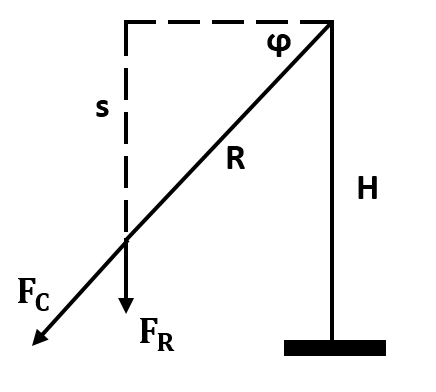
\includegraphics[scale=0.5]{2019-v2g-09-sol.png}
\end{center}
\probend